\section{Introduction}
\label{sec:intro}


\begin{figure}[t]
  \centering
  {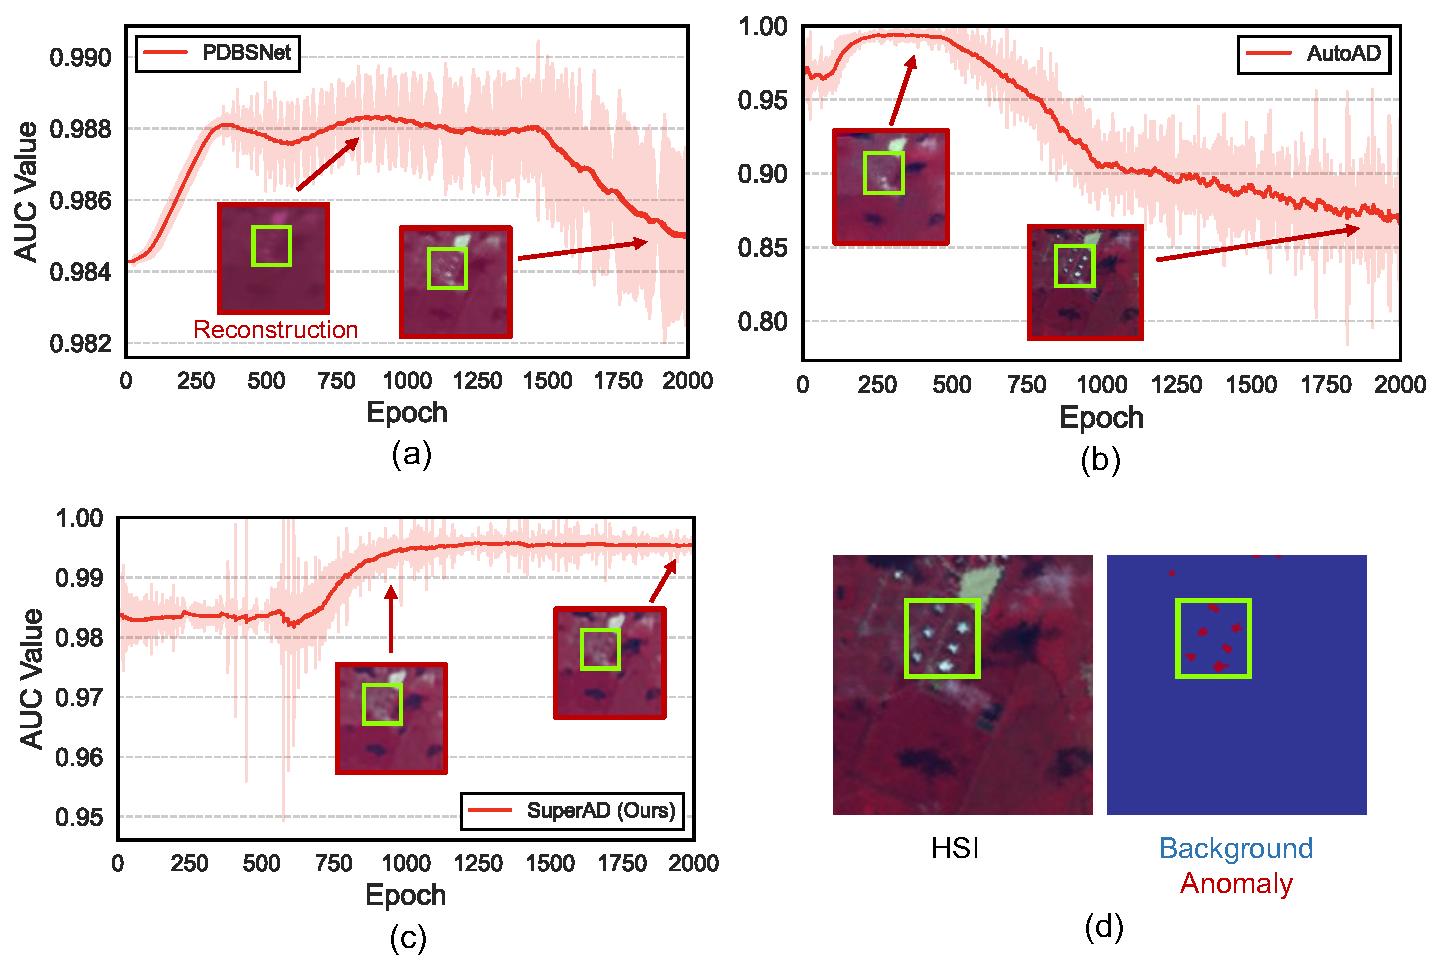
\includegraphics[width=1\linewidth]{Figures/PDF/teaser.pdf}}
  \caption{Comparison of reconstruction process across different models: (a) PDBSNet~\cite{PDBSNet}, (b) AutoAD~\cite{AutoAD}, and (c) our proposed SuperAD model. (d) shows the hyperspectral image and the groudtruth detection map. The fluorescent green rectangular regions highlight critical areas of interest that demonstrate the identity mapping phenomenon.}
  \label{fig:intro-imp}
\end{figure}



Hyperspectral anomaly detection (HAD) aims to identify pixels or regions in a hyperspectral image that exhibit spectral signatures significantly different from surroundings~\cite{9205919,su2021hyperspectral,bioucas2013hyperspectral}. Traditional methods for HAD have relied heavily on statistical approaches, such as the Reed-Xiaoli (RX)~\cite{RXD,1386510} detectors, collaborative representation (CR)~\cite{CRD,8561244} and low-rank representation (LRR)~\cite{7322257,liu2010robust}. These methods, while effective in certain scenarios, often struggle with the complexity and variability of real-world hyperspectral data, leading to suboptimal detection performance~\cite{7322257}. Compared to traditional methods, the advent of parameterized neural networks for self-supervised learning~\cite{AutoAD,PDBSNet,BiGSeT,BockNet,SMCNet,DirectNet,wu2024transformer}, has emerged as a promising approach in HAD. The core premise is that the background, comprising the majority of the image, can be approximated well by the model, while anomalies, being spectrally distinct, cannot be accurately represented by the learned background model~\cite{7322257,BS3LNet}. However, self-supervised models in HAD face a significant challenge known as the Identity Mapping Problem (IMP), which has been extensively mentioned in~\cite{DirectNet,BiGSeT,PDBSNet,BockNet,BS3LNet, rs16163036}. The IMP arises from the powerful nonlinear fitting capabilities of deep neural networks, which can lead to overfitting to the entire image dataset. As the complexity of the network increases or the number of training iterations grows, these models tend to reconstruct both the background and anomalies with high fidelity, resulting in imperceptible errors for anomalous pixels~\cite{9715082}. Despite the introduction of various models attempting to tackle IMP-related issues, a comprehensive analytical framework and a unified validation of solutions for IMP in the context of self-supervised HAD are still missing, lacking a holistic view of the problem. In this paper, we aim to fill this gap by conducting an in-depth exploration to the IMP. Specifically, we propose a unified framework (Super-AD) that describes the IMP from the perspective of network optimization, encompassing three key aspects: perturbation, reconstruction, and regularization. Each aspect corresponds to a specific solution that we introduce. Through extensive experiments on various hyperspectral datasets, we validate the effectiveness of our proposed solutions and demonstrate how they collectively contribute to overcoming the IMP.



To better understand the IMP and demonstrate the effectiveness of our proposed approach, Fig.~\ref{fig:intro-imp} presents a comparative analysis of area under the receiver operating characteristic curve (AUC) performance across different models when being optimized. Fig.~\ref{fig:intro-imp}(a) and (b) illustrate the AUC trends of two state-of-the-art self-supervised models, PDBSNet~\cite{PDBSNet} and AutoAD~\cite{AutoAD}, respectively. As training iterations increase, both models exhibit a common pattern: after reaching their peak AUC values, their performance gradually declines. This phenomenon directly reflects the IMP, where the networks' powerful reconstruction capabilities lead to overfitting, causing them to reconstruct both background and anomalous pixels with high fidelity (as highlighted by the fluorescent green regions in the reconstruction images). In contrast, our proposed SuperAD model, shown in Fig.~\ref{fig:intro-imp}(c), maintains stable AUC performance even with increasing iterations, demonstrating its robustness against the IMP. The reconstruction results further validate that our model effectively preserves the distinction between background and anomalies, preventing the reconstruction of anomalous pixels.


The main contributions of this work can be summarized as follows:

\begin{itemize}
    \item We present the first comprehensive framework that systematically analyzes the identity mapping problem in self-supervised hyperspectral anomaly detection, providing a detailed theoretical foundation and practical insights into this critical issue.

    \item We propose three key strategies to address the IMP: (1) superpixel-based pooling and uppooling operations to enhance spatial-spectral feature representation, (2) error-adaptive convolution to dynamically adjust feature learning based on reconstruction errors, and (3) online background pixel mining to improve model robustness against anomalies. Each component has been thoroughly visualized to demonstrate its effectiveness, including superpixel pooling visualization, pixel utilization visualization, and background mining process visualization.

    \item Extensive experiments on multiple hyperspectral datasets demonstrate the effectiveness of our proposed solutions in mitigating the IMP and improving anomaly detection performance compared to state-of-the-art methods. Our work provides valuable insights and a solid foundation for future research in self-supervised hyperspectral anomaly detection, offering a unified framework that can be extended and adapted to various related applications.
\end{itemize}
